\begin{figure}[htbp]
\centering
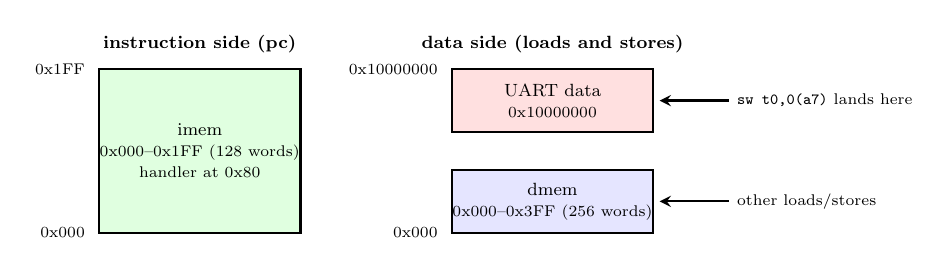
\begin{tikzpicture}[font=\footnotesize, >=stealth, scale=0.8, transform shape]
  % instruction side
  \node[font=\footnotesize\bfseries] at (1.6,6.4) {instruction side (pc)};
  \draw[thick, fill=green!12] (0,3.4) rectangle (3.2,6.0);
  \node[align=center] at (1.6,4.7) {imem\\ \scriptsize 0x000--0x1FF (128 words)\\ \scriptsize handler at 0x80};
  \node[anchor=east, font=\scriptsize] at (-0.1,6.0) {0x1FF};
  \node[anchor=east, font=\scriptsize] at (-0.1,3.4) {0x000};
  % data side
  \node[font=\footnotesize\bfseries] at (7.2,6.4) {data side (loads and stores)};
  \draw[thick, fill=red!12] (5.6,5.0) rectangle (8.8,6.0);
  \node[align=center] at (7.2,5.5) {UART data\\ \scriptsize 0x10000000};
  \draw[thick, fill=blue!10] (5.6,3.4) rectangle (8.8,4.4);
  \node[align=center] at (7.2,3.9) {dmem\\ \scriptsize 0x000--0x3FF (256 words)};
  \node[anchor=east, font=\scriptsize] at (5.5,6.0) {0x10000000};
  \node[anchor=east, font=\scriptsize] at (5.5,3.4) {0x000};
  \draw[->, thick] (10.0,5.5) -- (8.9,5.5) node[pos=0,right]{\scriptsize\texttt{sw t0,0(a7)} lands here};
  \draw[->, thick] (10.0,3.9) -- (8.9,3.9) node[pos=0,right]{\scriptsize other loads/stores};
\end{tikzpicture}
\caption{The two address maps of the ch08 SoC. The core has separate
instruction and data memories (a Harvard layout), each starting at
address 0. Only the data side has a carved-out address,
\texttt{0x10000000}, that belongs to the UART; any other store goes to
\texttt{dmem}.}
\label{fig:mmio08}
\end{figure}
